\Chapter{Making the Museum}{Clare Court}

When one looks back over the past eight years, or indeed over one's life as a whole, it is difficult to remember the exact moment at which certain events took place, and neither of us is quite sure of the exact time at which the idea of the museum first came to us. The germs of the idea must have been born in the first summer at Washford. We had been moving out, as I have already described, many items of furniture from the house - sideboards, cupboards, tables, chests of drawers - all these and many more, not forgetting of course the famous beds of solid oak. Whatever could be done with such an abundance and superfluity of furniture? A large load went to the saleroom, undistinguished items of no particular value for the most part, but many articles remained which could not be so summarily disposed of. For example there was the oak sideboard complete with \quotemark{top}, which had been made and carved by Uncle Lewis and elaborately decorated with a veritable cornucopia of wooden fruit surmounted by his own initials L.H.C. skilfully intertwined. What was to be done with it?

Uncle Lewis had died childless so there were no direct heirs to take an interest in something so intensely familial. The base part was functional, and could conceivably be used as a sideboard, but the whole design of the piece was indelibly stamped with the style of the 1920s period. Besides we already had a modern beech sideboard and I had no intention of replacing that with a dark oak model, however lovingly carved and however splendid an example of Uncle's art it might be. It was already a full time occupation dealing with the many articles which had been made (or more often begun and never completed) by Glyn's Father without including the handiwork of Uncle as well. If we continued at this rate we might as well throw the field open to the whole of the rest of the family including their relations - or so I argued! 

\quotemark{And how about Grandfather's table?} \\
\quotemark{Which table do I mean, you say? Or which Grandfather?} \\
\quotemark{Well, one of the Grandfathers. Does it matter much anyway?} \\
\quotemark{Well you know the table I mean. It's been out in the shed for years.} \\
\quotemark{Oh yes. I remember. Kathie gave it to us, but we aren't to get rid of it - she wants to know where it is.} \\
\quotemark{Use it? No, of course, she never used it. She had lots of tables.} \\
\quotemark{What did she keep it for then?} \\
\quotemark{Because it was Grandfather's, of course!} \\

In the face of such crushing arguments what could one do?

So we put these sideboards and tables out in the building which we call the Toc H. Most of the old shoes had been cleared away by this time, and the downstairs room with the cobbled floor received two heavy oak cupboards and Jim Slade's sofa. This particular item had always irritated me beyond measure, I grew up in a period when Victorian furniture had gone completely out of fashion and I could not for the life of me think why my parents-in-law kept this ugly horsehair couch in their house. The room in which it was stored (though \quotemark{stored} is perhaps too grand a word, they had more likely just put it there one day, and left it) was the \quotemark{middle} room of which I have already spoken. This was one of the rooms which had been allowed to get into a very poor state of repair, and indeed it had presented a sorry spectacle for many a long year. It had been painted once when the house was built, with greenish blue distemper, but so long ago that there were patches of discolouration all over the walls, and as if this were not enough the ceiling was badly cracked and more grey than white. Over the fireplace the rain had been leaking in for a decade or two and the plaster was flaking off. The sofa stood forlornly along one partition. Not only was tile horsehair upholstery sadly dilapidated, and one leg broken, but to complete the sorry sight, the cushions had been encased in an old mail bag to prevent the stuffing from falling out. As the sofa was never used for sedentary purposes, over the years Ada had gradually filled up the space on the seat with cardboard boxes containing odds and ends of various sorts.

I had often said that if the day came when we ever inherited the house, the first thing that I would do would be to get rid of the sofa! However, when the time did come one's feelings were very different from what one had imagined they might be, and somehow it no longer seemed quite so clever or satisfying merely to throw away a piece of broken old furniture. Besides, Glyn knew a little more about its owner than I did and did not like to see it consigned to the rubbish heap. So the sofa joined the sideboard, and a heavy oak Elizabethan style cupboard in the Toc H.

When the time came for us to be moving all of our own furniture into the house the problem of space was becoming more and more pressing - until suddenly one day I had an idea. Instead of just keeping so many articles which for various reasons, mainly sentimental, could not be got rid of, why not concentrate them all in one building, using the spare furniture to display the items? There was plenty of wall space to hang pictures, spare tables on which to arrange exhibits and glass fronted cupboards in which to put more valuable or fragile articles. The unwanted sideboards and chests also had drawers in which to stow things which would not be exhibited but which have a certain interest. Once the idea had been born, we both embraced it with enthusiasm. I must admit that one of the principal motives which activated me at the beginning was the desire to set aside one definite place in which to store all the old things. I am naturally a fairly tidy person - not fanatically tidy, but I do like having things in order. From the very moment that we definitely started working with a museum in mind, everything started to fall into place. Of course a prodigous amount of energy had to be expended on the physical removal of the articles and assembling them all in the two rooms. For example, Grandfather's sewing machine had been standing for years in the wash-house at the rear of the premises. It is extremely heavy, the base being made of cast iron and the work table of some heavy hardwood. I found an old tin of bicycle enamel and smartened up the iron work a little, splashing some varnish on to the wood. We managed to manipulate the machine on to an old pushchair belonging to one of our children, and with a great deal of pushing and shoving succeeded in getting it around to the Toc H and up the not inconsiderable step. Occasionally we are asked if we would be willing to lend it for exhibition - unfortunately the answer is \quotemark{No!} - we are very sorry, but prospective viewers must come to the machine and not vice versa!

Having got some furniture into the rooms, we felt we had at least got a rough foundation on which to build. Upstairs was more of a problem, as the room is quite large but we did not feel equal to the task of heaving solid oak sideboards and the like up the stairs. To begin with we spread an old carpet and then arranged a few of our spare tables (about four altogether, not counting several that had been sent to the sale room!) This started to look promising, and Glyn then had the idea of using the old mahogany counter from the shop. Glyn's father had always prized this wood very much, as he had purchased it at Watchet harbour when a ship called the \quotemark{Fox} was being broken up, I always imagine it as having formed a table or work top for a steward or in the officers' mess, and it certainly used to look very nice in the shop when well polished. This turned out to be quite a successful idea as the counter top, being in two pieces, stretched around two sides of the room. Admittedly the legs were not quite on a par aesthetically with the top, consisting as they did of old washstand bases and similar humble supports. Once this was up, we were able to put the glass fronted cupboards and bookcases on the top - these were reserved for more precious and fragile exhibits. In odd corners, we placed various odd chairs to fill up the spaces.

We were painfully aware while doing this that the room badly needed decorating, and we somehow found the energy to splash some emulsion paint on the worst parts of the walls. The windows were in a bad way and it did not exactly help matters when, in an enthusiastic access of cleaning feruour, I cast one open and the whole frame fell out completely, smashing to pieces on the ground. This was a minor disaster but Glyn somehow managed to screw the pieces together rather amateurishly and more or less nailed the window back into place.

Once the donkey work was over we were able to start actually bringing things in and arranging them. This was far and away the most enjoyable part, though even this involves a great deal of walking about. It is surprising how many miles one covers simply going back and forth into the house to fetch scissors, drawing pins, cards, felt tip pens, hammers, dusters, polish, window cleaner, Brasso and all the dozens of accessories necessary to make the exhibits look fairly presentable.

All this would be very well on its own, but we were encumbered with the shop and quite often had to run down to it to see to a customer, quite apart from keeping the home running smoothly and children fed and reasonably clean. We knew that unless we had a deadline to work to, we would never be ready in time so we fixed an opening date and the last two days were really hectic. When reading the Duke of Bedford's book \quotemark{A Silver Spoon} I could not help smiling at the similarity of our experience with his! He describes how he and his family worked themselves into the ground preparing for their first opening, even washing and cleaning priceless tea sets and solid gold dinner services by hand. When the visitors came and were asked what they had liked best, one said \quotemark{That lovely set of brass}!

Glyn took on the job of arranging all the photographs, an extremely difficult task as there were so many of them. They had mostly been collected by Uncle Lewis, and he had usually written on the back of them who, what or where, which proved very helpful. It is of course quite impossible to display them all, but is a never-ending source of interest to visitors, especially those who remember the valley as it was years ago. Sometimes we are visited by people whose parents or grandparents were born in the district, and occasionally we have been able to show them a photograph of one of their relations, or the cottage in which they lived. (The main problem with displaying photographs, apart from their tending curl up and pop out of the mounts, is the effect of daylight on them. Unfortunately we were too busy to think about such things when we first arranged our museum and sunlight did cause some of them to fade. So we fixed up old curtains and try to keep out the daylight when the museum is closed, and this has worked very well on the whole.)

The girls and I tackled the task of arranging the Edwardian dolls. For years they had been lying under Ada's bed in an old suitcase, and she had occasionally shown them to the children. They have rather a pleasing family connection as the two best ones belonged to a cousin who still lives in the village, and they were dressed for her as a little girl by Ada when she was a young woman, Ada always used to say that she could happily spend all her spare time making dolls clothes as she loved doing it so much. As a young woman she delighted in any work that required very small stitches, tiny buttons and minute tucks. This was a legacy her last year at school when hours spent sewing was considered a suitable occupation for a working class girl. Unfortunately Ada did not quite fall in with the pattern that was probably expected of her - plain sewing did not appeal to her at all and as far as I can remember she never made any garments at all for herself. But the dolls were very well equipped and the hats she had plaited out of raffia. Not only did we have their spare underclothes, but a whole box full of little petticoats, chemises, spencers, and the like which must have belonged to her departed sisters and relations. Most of these clothes were very soiled, and as they appeared to be made of strong cotton I tentatively soaked and boiled them in a well-known brand of detergent. After this operation they shone forth in pristine whiteness. The more delicate articles I washed carefully in soap flakes and these too responded very well. After this little venture I wrote to the manufacturers of the detergent informing them of the results of my tests but they were not impressed and I did not even receive a free packet of soap powder for my pains. So much for big business!

One of the dolls had a broken leg, china of course - but this was easily repaired. Rather touchingly, although she must have been broken for at least fifty years, the owner having long since grown up, the pieces had been carefully preserved in an old shoe box and fitted together perfectly. We had never done anything like this before but the results seemed fairly satisfactory. We finally arranged them in an old glass cupboard, sitting down on velvet couches, (in reality my children's building bricks covered with a piece of old velvet curtain) and they appear to be having a little tea party with a doll's tea set. The finishing touch was given when our cousin came in and saw them, for she was able to tell us their names, Lily and Dorothy. 

The boots and shoes presented quite a problem. We felt they would be interesting and they also came in useful for filling up odd spaces. However, they had been lying around for so many years that they needed sorting out and cleaning, and this alone was a major task. Displaying them too had its problems - boots and shoes stand up quite well, but taller models have to be padded with paper to make them stand up. I labelled them hopefully with approximate dates which are very inaccurate - it seems difficult to place some of them to within a year or two as most books on the subject only go up to the beginning of the twentieth century, which is when most of ours begin. Occasionally an old lady or gentleman will come in and recognise a style that they themselves wore when younger and this is very helpful in trying to fix an approximate date. Gradually no doubt we shall succeed in filling in the missing background information to some of our exhibits, but as we do not set out to give an accurate historical catalogue but rather to set the atmosphere of a period, we do not think it is a life and death matter to have a few inaccuracies in our assessment of dates and so forth. Apart from anything else, it gives visitors great pleasure to be able to give us information, and this surely should he one of the functions of a museum - to stimulate discussion and communication. We have often noticed that if there is one thing that many people enjoy doing, it is correcting you if you are wrong.

\begin{figure}[]
     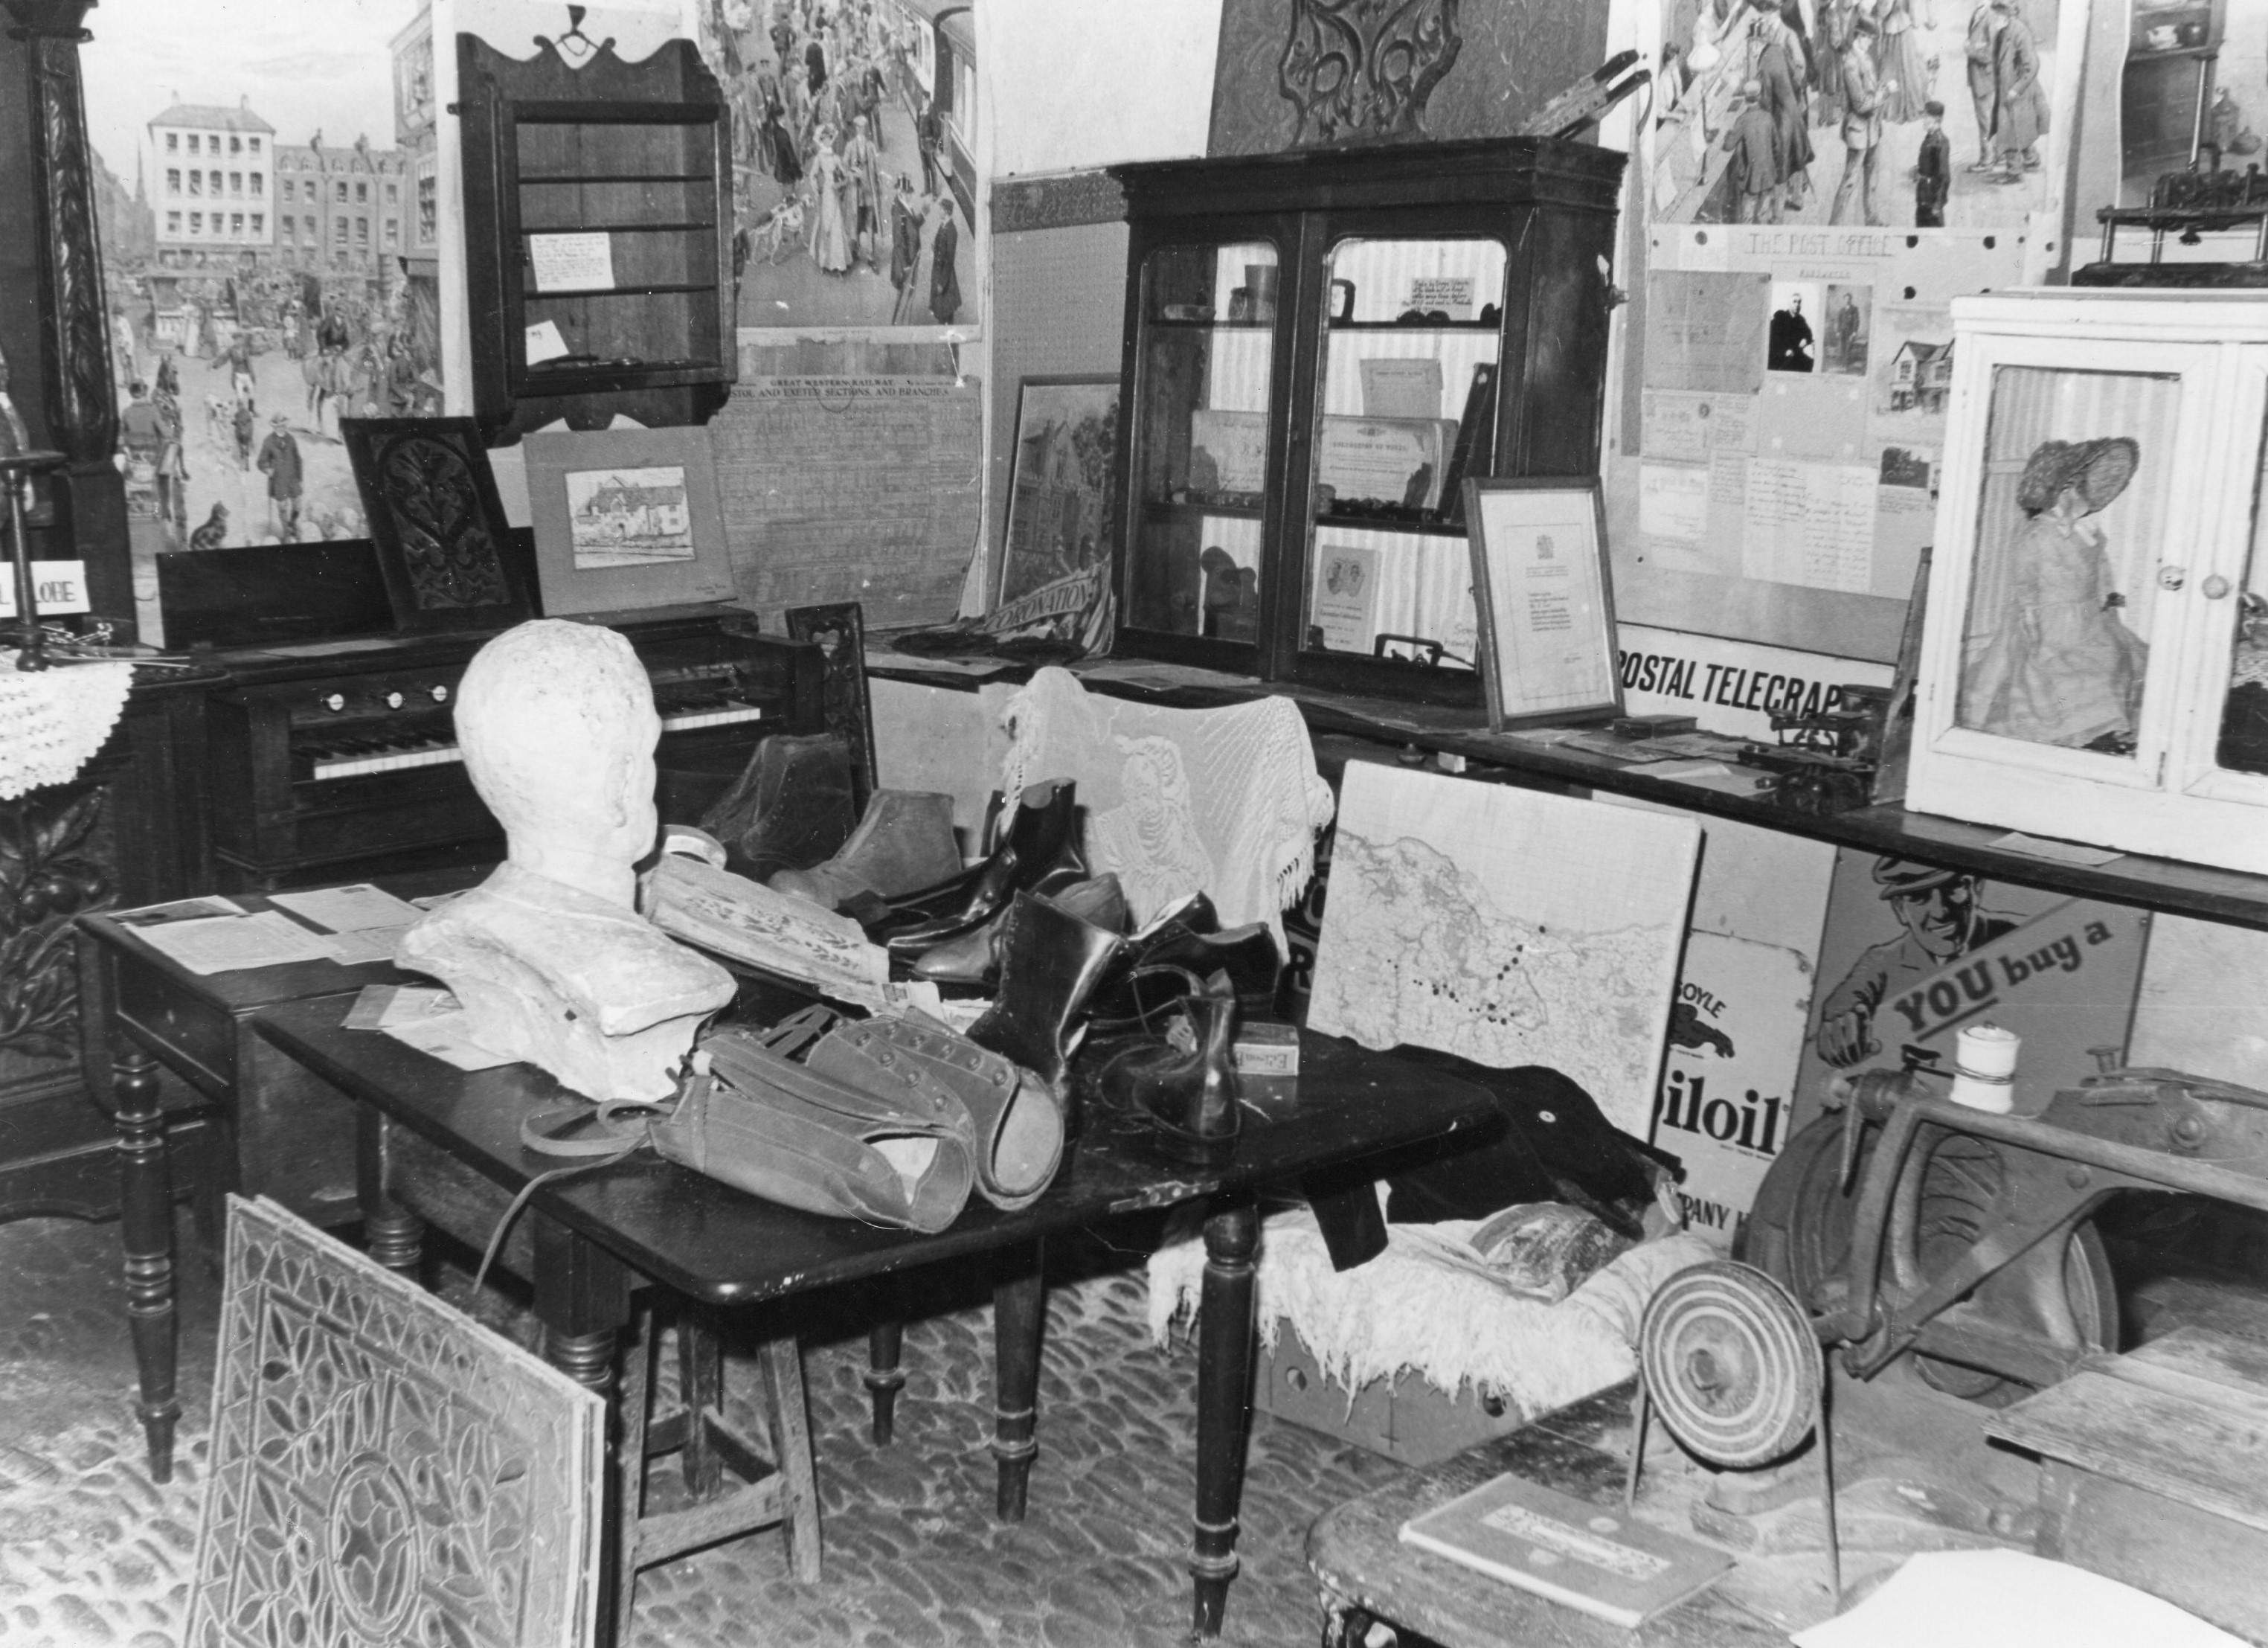
\includegraphics[width=1\textwidth]{figures/Museum2}
     \caption{A view of the Museum collections. A collection of artwork, shoes and machinery can be seen.}
     \label{fig:Museum2}
\end{figure}

As the time grew shorter towards the advertised opening of the museum the pace quickened to a frantic gallop. Many local people were now aware of what we were doing, as we had gone to the expense of having bills printed. (These cost five pounds - we did not repeat this rather extravagant gesture.) Then the local press sent along a reporter and we suddenly felt the excitement mounting, and an earnest determination to achieve the best possible result with the limited means at our disposal. When the reporter came to see us we were still hopelessly unprepared - everything was lying around in confusion and any resemblance to a museum (or \quotemark{exhibition} as we were calling it) was purely nominal. Nevertheless he was impressed and wrote a very helpful and appreciative article in our local journal. 

\begin{figure}[]
     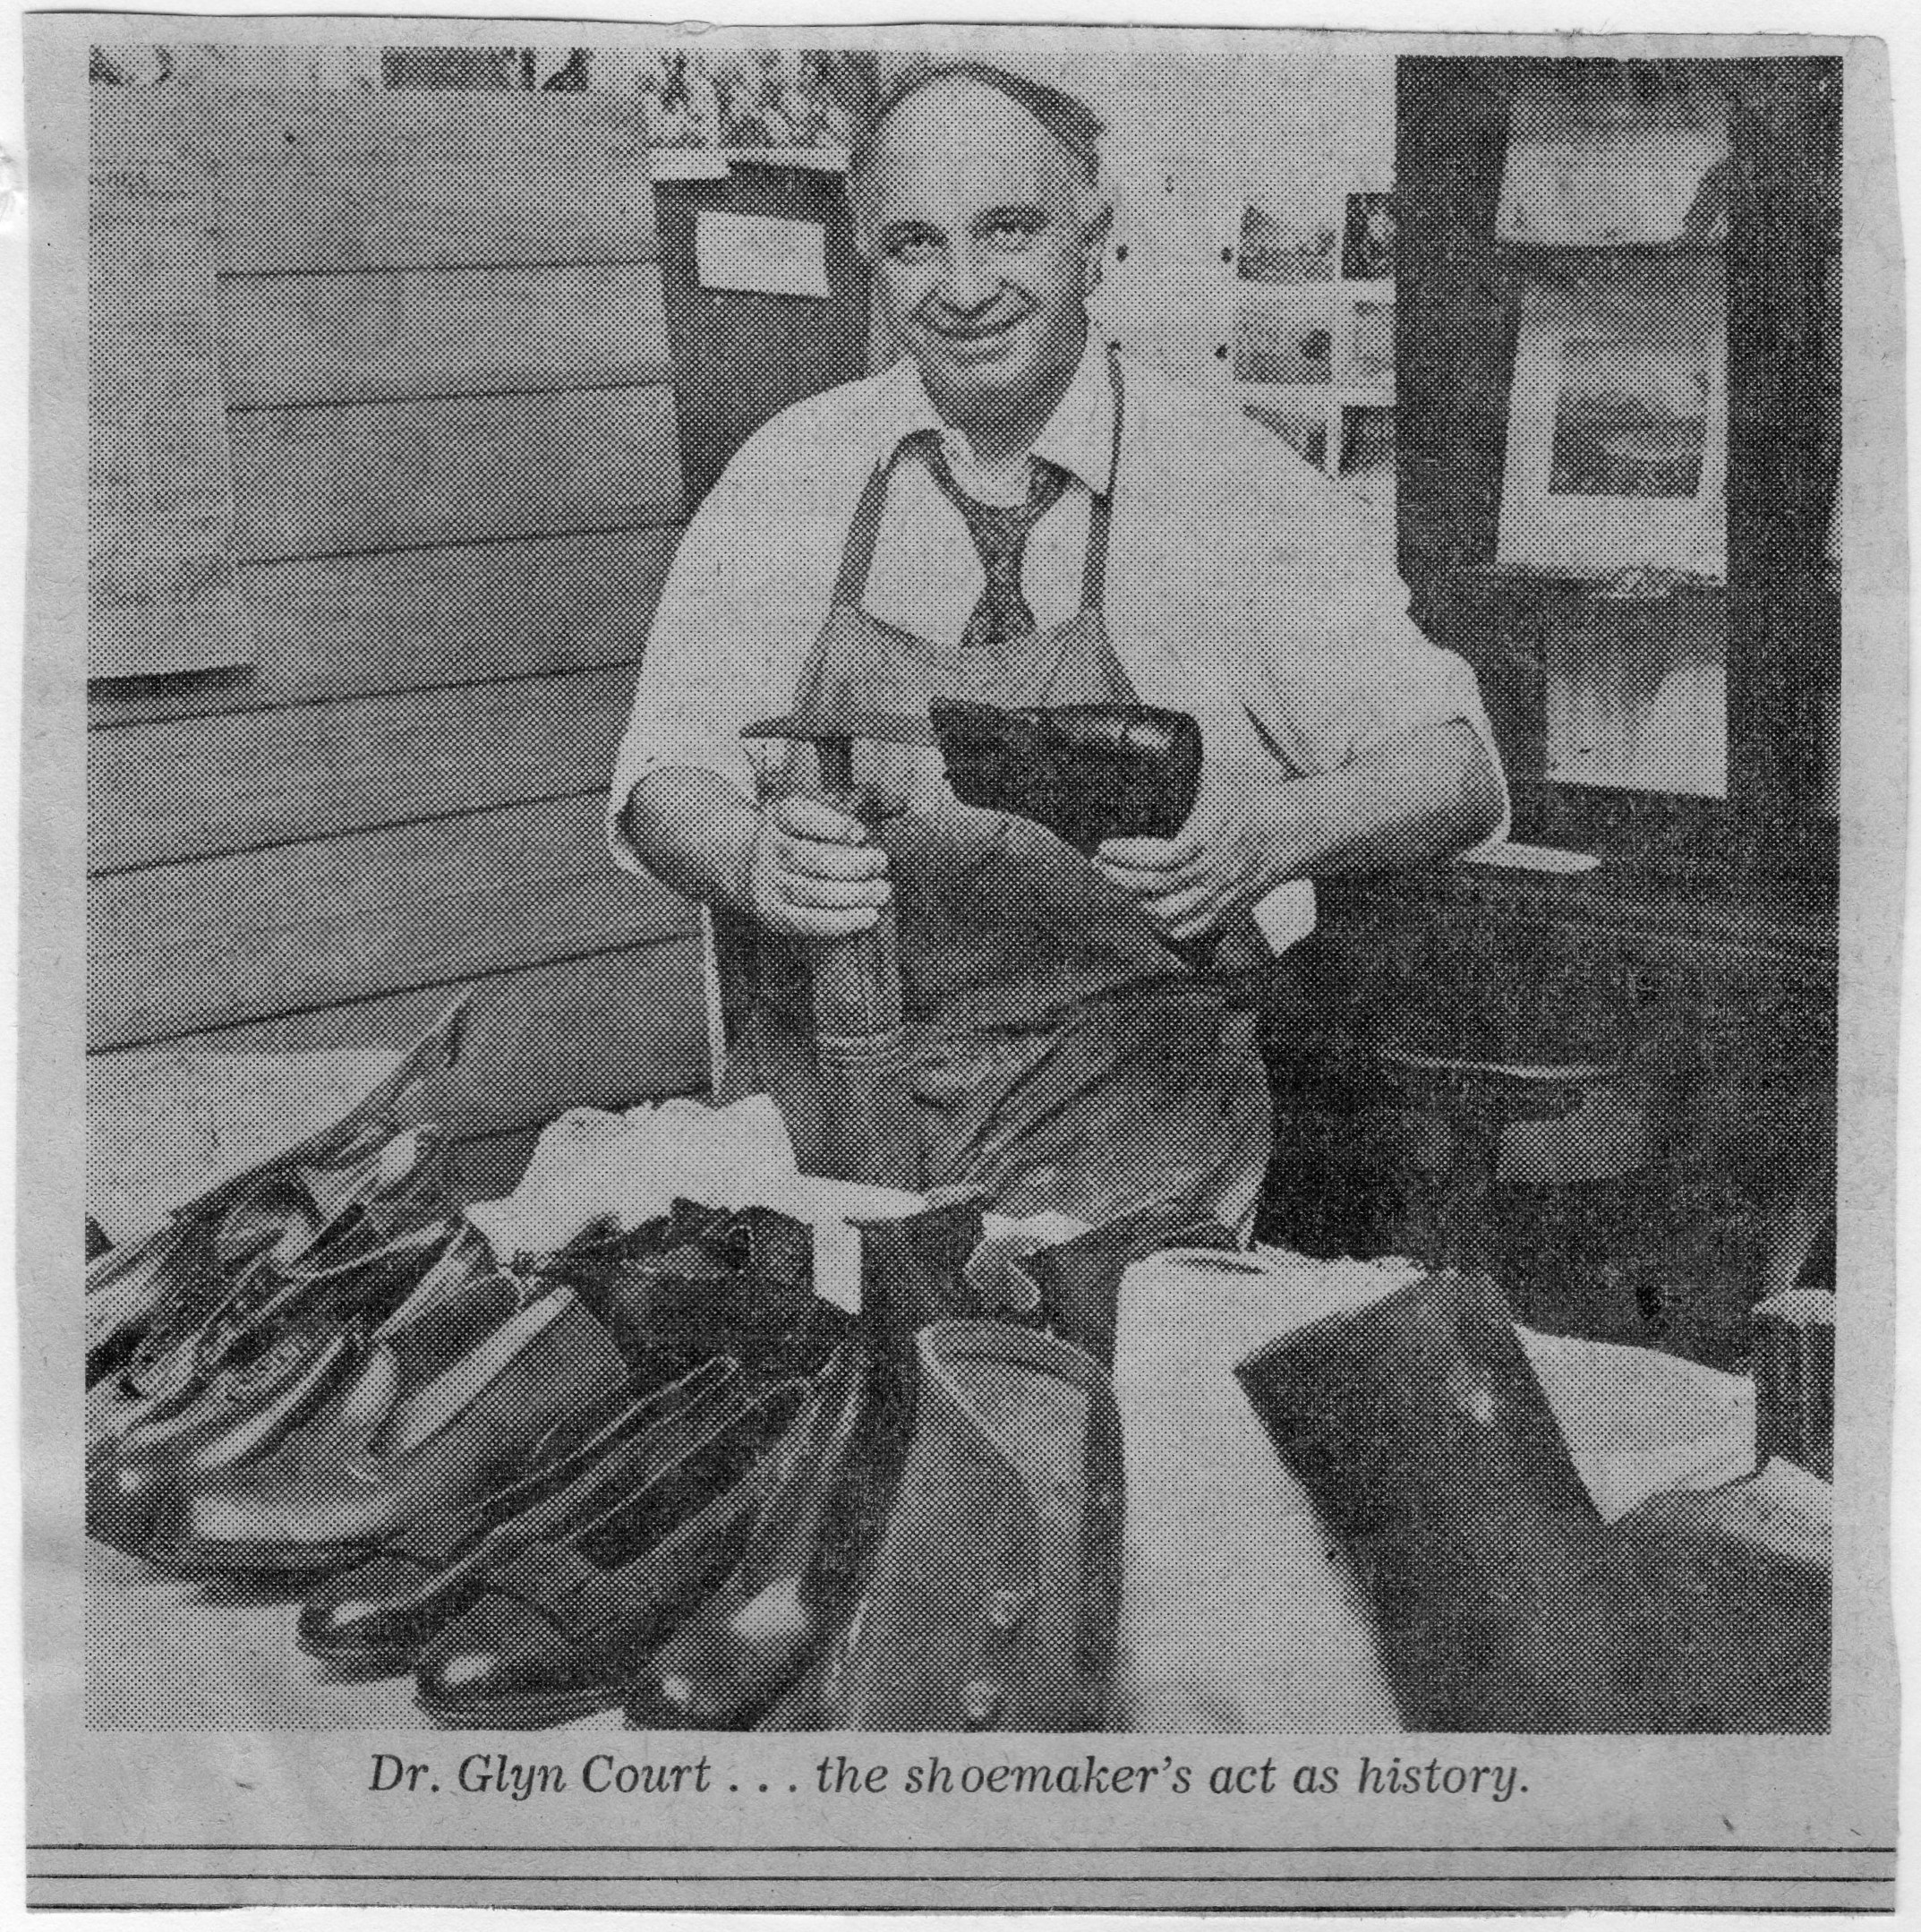
\includegraphics[width=1\textwidth]{figures/Museum}
     \caption{Newspaper coverage of the opening of the museum}
     \label{fig:Museum}
\end{figure}

On the last evening we stayed up most of the night getting things arranged and making tickets. It is unbelievable how long it takes to write out all the labels - but it is an essential part of the work. In my haste I dropped a shoe box full of Edwardian dolls and broke one of the heads. Shame on me! However, I think this was the only casualty.

The first day started very well - people came in rather hesitantly at first, but by the end of the week we had shown about a hundred people around. Some of the visitors had read about our venture in the local newspaper, or seen the home made notices which we had fixed up. Others had known the family for years and came out of a mixture of sentiment and curiosity. About half way through the week, we were visited by Independent Television and had the thrill of seeing ourselves turning the handle of the sewing machine and displaying the dolls.

One of the snags about our little collection (really \quotemark{museum} is such a grand word, but somehow we have got into the habit of this designating it) is that, owing to the very strong family ties and connections of most of the exhibits we feel rather hesitant about asking for help from volunteers. The museum is unique in that all, or nearly all, the exhibits were collected by one family - not wealthy landowners, commissioning works of art to beautify their houses, but ordinary working folk. Often, the reasons for keeping the articles were sentimental but many things were saved by Glyn's Father out of a love of the quaint and curious and because he could not bear to see them thrown away. A charcoal smoothing iron falls into this category. We have been given a few articles which were used at various villages in the parish, and could probably acquire a great deal more if we had the time and energy and money to devote to collecting it, but we feel that the museum would not be quite the same. Its unique character and flavour, untidy and dusty though it frequently is, is given by the characters and occupations of the members of the family. Take for example the family business - bootmaking allied to a Post Office. That in itself is an unusual combination, and one which I do not think I have ever seen anywhere else. Methodism, (in the particular brand which moved the spirits of our ancestors, the Bible Christian Connexion), the West Somerset Mineral Railway, the coming of the bicycle and the motor car, all these had their influence and have left their mark on the museum.

\begin{figure}[]
     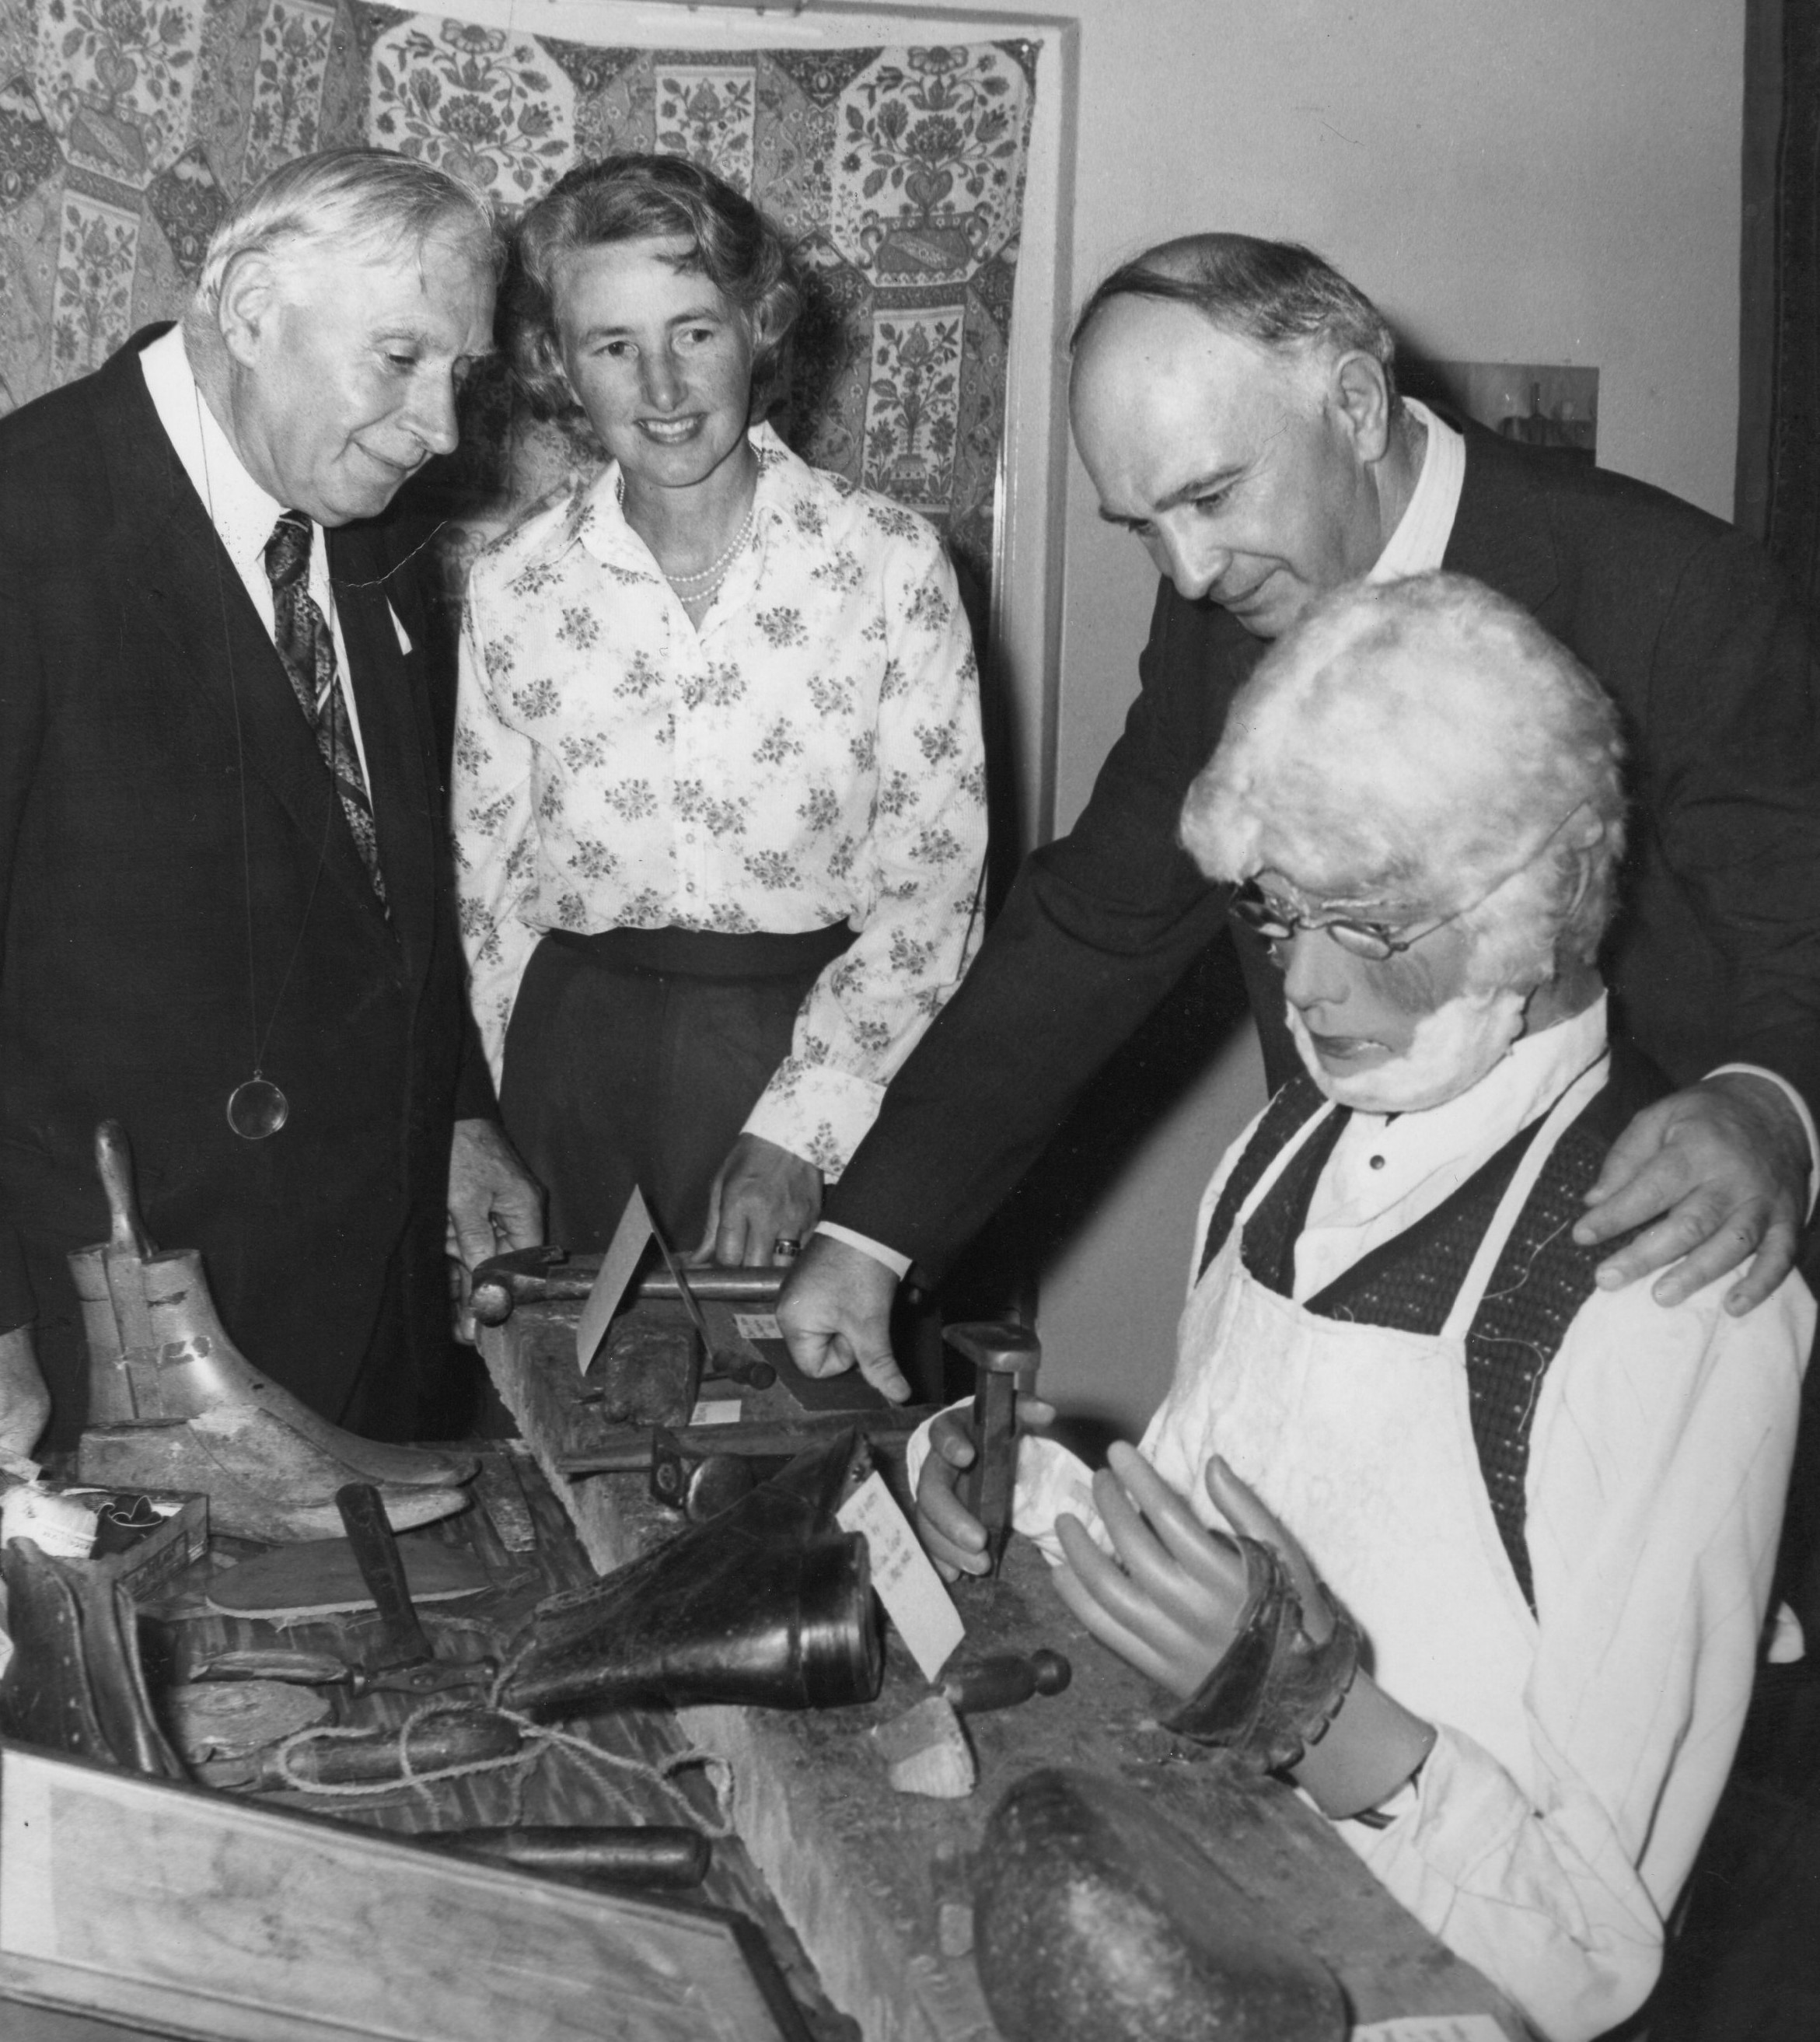
\includegraphics[width=1\textwidth]{figures/SomersetLife}
     \caption{Parts of the museum were occasionally used for external exhibitions. Somerset County Council chairman, Mr. William Knowles, opens \quotemark{Somerset Life a Century Ago} which was presented to help celebrate Minehead Festival}
     \label{fig:SomersetLife}
\end{figure}

For this reason, the very uniqueness, albeit a trifle inbred, of our collection, renders it difficult for us to seek official aid. We love showing people round, but it is very time consuming and so are not able to open the museum very often. So until we can do the job really well, we soldier on alone, keeping the daylight and rain out as well as we can, and lighting a paraffin stove in the winter months. The important thing is to preserve it all. Restoration, air conditioning and so forth can come when our fairy godfather visits us some time in the future. Until the happy day when, retired from teaching and politics, we sit at home and wait for people to come and visit us, we try to open the museum for a week during the school summer holidays. It is very hard work, cleaning, tidying and sticking up all the photographs which have fallen off, and a week of this is usually quite enough. In between whiles we are happy to show people around if they give us a little warning. We have been privileged to meet some very delightful folk when throwing our doors open to the public. The very first day of the opening in 1968 a young Canadian couple came in. Their name was Burnett, an old established Washford name, and it was good to feel that our little corner of Somerset had a link with distant North America. We have had visitors from many different countries, and the majority of them have devoured every word of information we have given them. Often, the visitors tell us very interesting facts which increase our own knowledge. One most rewarding factor is the pleasure that it gives people to see again some object which reminds them perhaps of their childhood or their apprenticeship or perhaps the home of their own grandparents. For example, one gentleman came in who had served his apprenticeship as a bootmaker in a factory in Leicester. He immediately spotted the shoe finishing machine - not one of ours, actually, but given to us by an elderly bootmaker in Watchet. Within seconds he had readjusted the bands which drive the various cogs and wheels, and had soon polished all our shoes for us. We all enjoyed this very much. Then there was a young married couple who came in and listened politely and as we thought, coldly, to our little peroration. I thought the wife was bored but it turned out that her hobby was wood carving! We have numerous examples of the woodcarvers art in various stages of completion, and also a set of wood carving tools. These were lying about in a corner, as I had not attached much importance to them since removing them from the old washstand where they had lain for years. To our amazement the young woman in question informed us that the tools were valuable - upon which we promoted them to a glass cupboard! A couple of years later I was showing a middle-aged man round who turned out to be an expert on old tools.

Within seconds he had whipped out his pocket magnifier and was examining the marks on the handles of the implements. They showed crossed rifles, the old sign of the War Office, discontinued in the 1890s. He suggested that Glyn's Father had probably bought the tools second hand, as they would have been surplus to Army requirements when wooden gun carriages gradually became obsolete. We remembered then that Ada had often told us how William had saved up his money in order to buy each tool, with the same dedication as a golfer collecting a set of clubs. Wages were low in the 1890s and possessions treasured, and this explained why Ada had always kept those hard earned tools so carefully after William's death.

Occasionally we get visitors who also keep a shop, or are boot repairers, and they too recognise the fittings and appurtenances of the bootmaker's trade. The old shoes are always popular. Gentlemen love to reminisce over the dancing pumps and recall how they used to take them to dances in a brown paper bag in their pockets. As a footnote to this item it is interesting to note that the Village Hall at Roadwater still sports a much-treasured notice \quotemark{Dancers are requested to remove their Boots}.

The crystal set is not particularly old - it is one that Glyn had when he was a lad, but it also evokes many memories among the old and not-so-old. We have repeatedly found that the things which people most enjoy looking at are articles which have passed out of use in their own lifetime - often very simple items. Take, for example, those round leather studs which used to be nailed to the soles of football boots. And the wartime collection, though small - a chance assembly of ration books, coupons, with a gas mask or two, is always tremendously popular. (The gas masks were out in the washhouse, still in their original boxes. Children love them!)

One of the cupboards is filled with all the small pieces of bric a brac, many of which are of no particular value, but interesting. For example, there is a piece of broken tile from Cleeve Abbey. My children found it in the stream when paddling around a year or two ago - the Water Board had just been engaged in flood prevention work, and no doubt the piece of tile had been washed out of the newly excavated river bank. Lying about the garden, as I have mentioned elsewhere, are numerous carved and dressed stones which obviously must have been pillaged from the Abbey many years ago. Apart from these chance remains we make no attempt to vie with the Ministry of Works in their presentation of the Abbey's history, after all, they are the professionals and have far greater resources at their disposal than we have. Our two worlds are very different and we have not many points of contact, but perhaps when the happy day arrives when the main road is removed from our midst, there will arrive a new era in which people on holiday can stroll pleasantly from one museum to the other. We do, after all, within the space of a few hundred yards, present two totally different aspects of life as it has been known in our valley. Perhaps there was even a member of our family in those distant days who visited the Abbey to repair the Monks' footwear, or carve pews for the church. Who knows? Although at the time of writing there is no record in Parish registers of a Court earlier than 1750, it is as likely as not that the family was already established in the area. Country folk, after all, did not move around very much, and even in these days, as a casual glance at the telephone directory will tell, just how localised some family names are.
